\Problem
{ناحیه‌بندی فرکانسی صورت پذیرفته توسط \lr{ITU}}
{
دسته‌بندی این باندهای فرکانسی با توجه به فرکانس، کاربرد آنها و موفعیت جغرافیایی صورت گرفته است.

این سازمان ابتدا زمین را به سه ناحیه تقسیم کرده است که ناحیه اول شامل اروپا، آفریقا، روسیه، بخشی از خاورمیانه و کشورهای غربی خلیج فارس است.
ناحیه دوم شامل قاره آمریکا است.
ناحیه سوم شامل کشورای شرق آسیایی و ایران، کشورهای جنوب شوروی و کشورهای اقیانوسیه است.
طبق یکی از قطعنامه‌های
\lr{WRC}
هر ناحیه مجموعه ای از تخصیص‌های فرکانسی را در اختیار دارد.

\begin{figure}[H]
    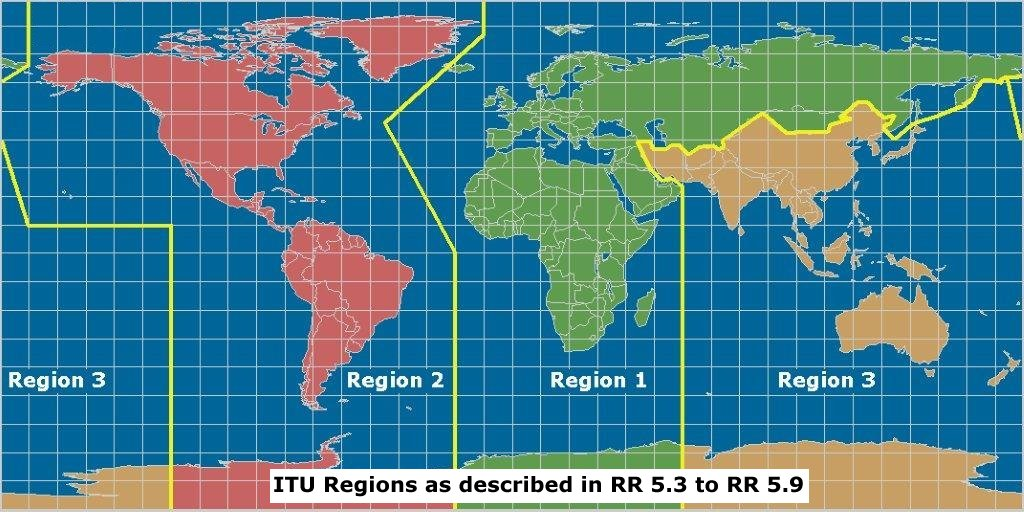
\includegraphics[width=12cm]{Images/ITU_Regions.jpg}
    \centering
    \caption{\lr{ITU Regions}}
\end{figure}
}
